\documentclass[12pt]{beamer}
\usetheme{Madrid}
\usecolortheme{default}
\usepackage[T2A]{fontenc}
\usepackage[utf8]{inputenc}
\usepackage[russian]{babel}
\usepackage{graphicx} % Required for inserting images
\usepackage{wrapfig}
\usepackage{caption} % заголовки плавающих объектов
\usepackage{subcaption}

\captionsetup[table]{justification=centering}
\captionsetup[figure]{justification=centering}
\addtobeamertemplate{block end}{}{\vskip -\smallskipamount}
\beamertemplatenavigationsymbolsempty
% \setbeamertemplate{footline}[text line]{%
%     \parbox{\linewidth}{\vspace*{-8pt}\hfill\hfill\insertframenumber\,/\,\inserttotalframenumber}}
\usepackage{etoolbox}
\AfterEndEnvironment{figure}{\vskip-1ex}
\setbeamertemplate{caption}[numbered]
\setbeamertemplate{navigation symbols}{}
\title[Волноводы]{Электромагнитные волны в волноводах}
\author{Пазов Тенгиз, Симухин Егор}
\date{Декабрь 2024}

\begin{document}


\maketitle

\begin{frame}{Вступление}

В данной работе изучается распространение и отражение волн различных сигналов СВЧ - диапазона в волноводе.
\end{frame}

\begin{frame}{Цели и задачи}
    \begin{block}{Цели}
        \centering
        Ознакомиться с методами получения и анализа электромагнитных волн СВЧ - диапазона.
    \end{block}

    \begin{block}{Задачи}
        \item 1. Изучить структуру волн при частоте выше критической
            \begin{itemize}
                \item Определить длину волны СВЧ-сигнала в волноводе
                \item Определить характер детектирования в волноводе
                \item Определить коэффициент отражения
            \end{itemize}
        \item 2. Исследовать затухание волн при частоте ниже критической
            \begin{itemize}
                \item Измерить коэффициент затухания
            \end{itemize}
    \end{block}

\end{frame}



\begin{frame}{Экспериментальная установка}
    \begin{figure}
        \centering
        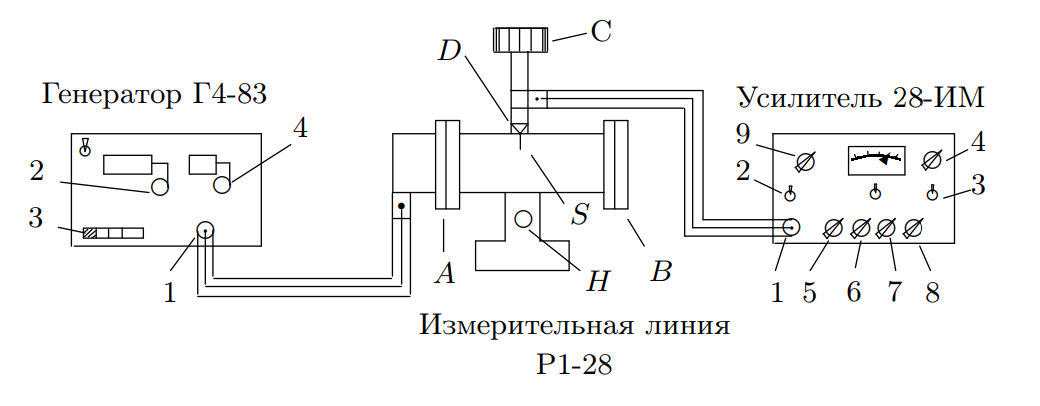
\includegraphics[scale=0.4]{fig2.PNG}
        \caption{Схема экспериментальной установки для измерений при частотах выше критической}
        \label{fig:enter-label}
    \end{figure} 
\end{frame}

\begin{frame}{Экспериментальная установка}

    \begin{figure}
        \centering
        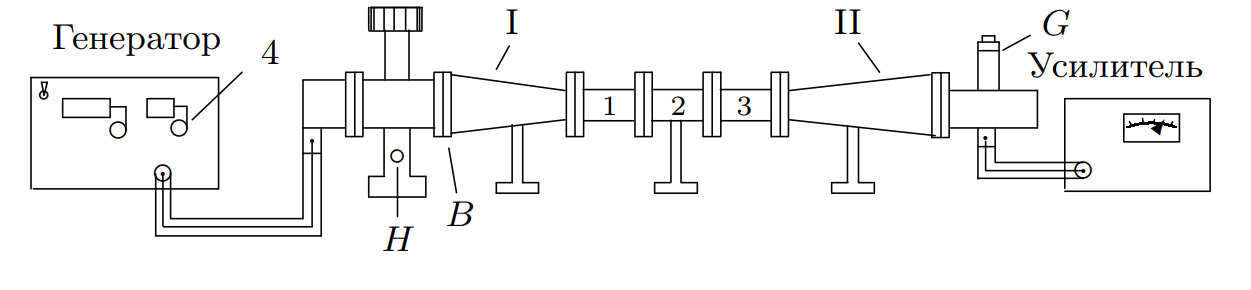
\includegraphics[scale=0.35]{fig3.PNG}
        \caption{Схема экспериментальной установки для измерений при частотах ниже критической}
        \label{fig:enter-label}
    \end{figure}
    
\end{frame}


\begin{frame}{Экспериментальная установка}

    \begin{figure}[!h]
        \centering
        \begin{subfigure}{0.5\textwidth} % Задаем ширину подфигуры
            \centering
            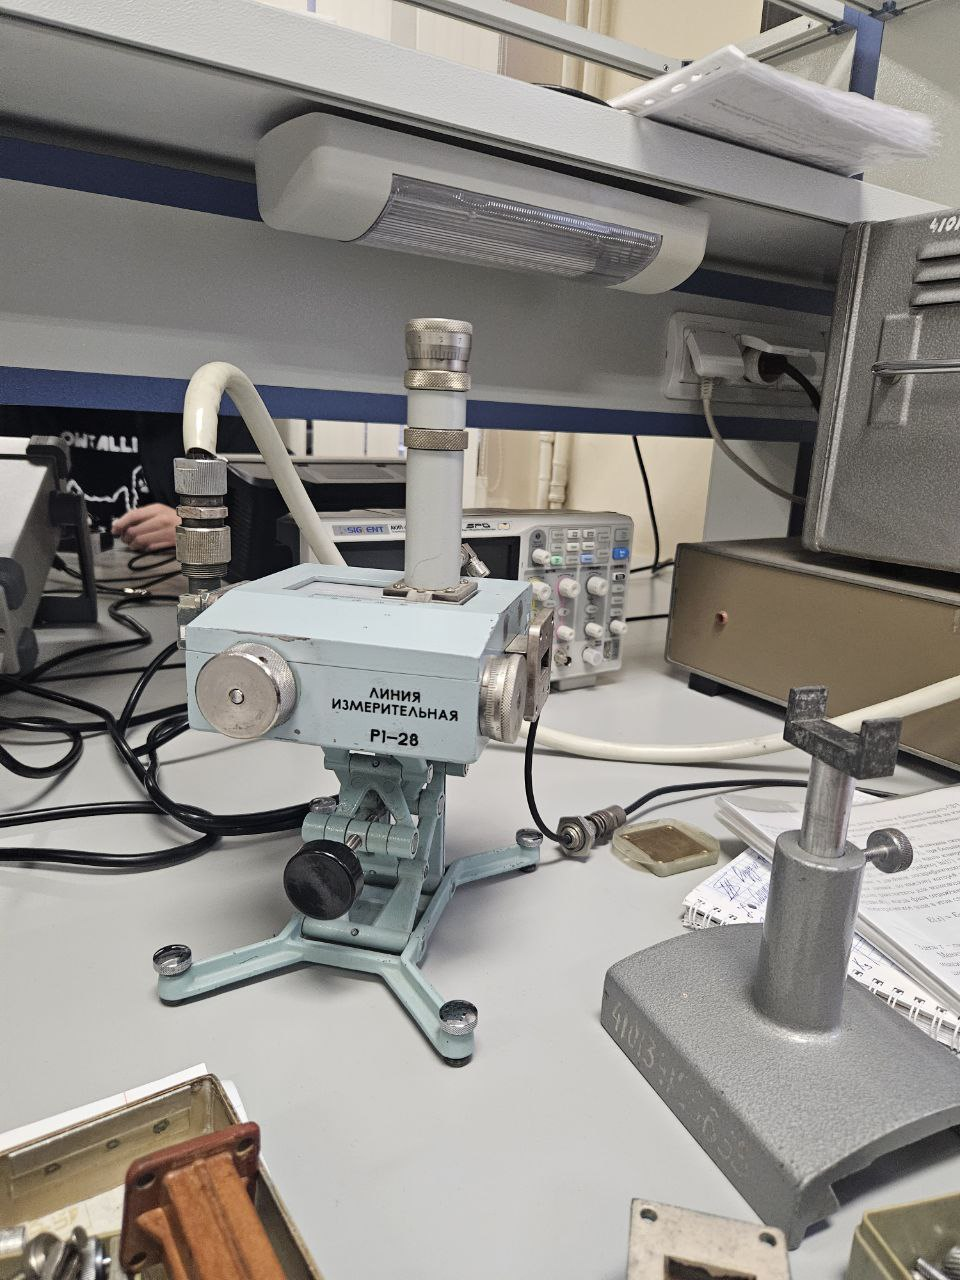
\includegraphics[scale=0.08]{photo_2024-12-24_17-45-34 (2).jpg}
            \caption{Измерительная линия}
        \end{subfigure}
        \hfill
        \begin{subfigure}{0.45\textwidth} % Задаем ширину подфигуры
            \centering
            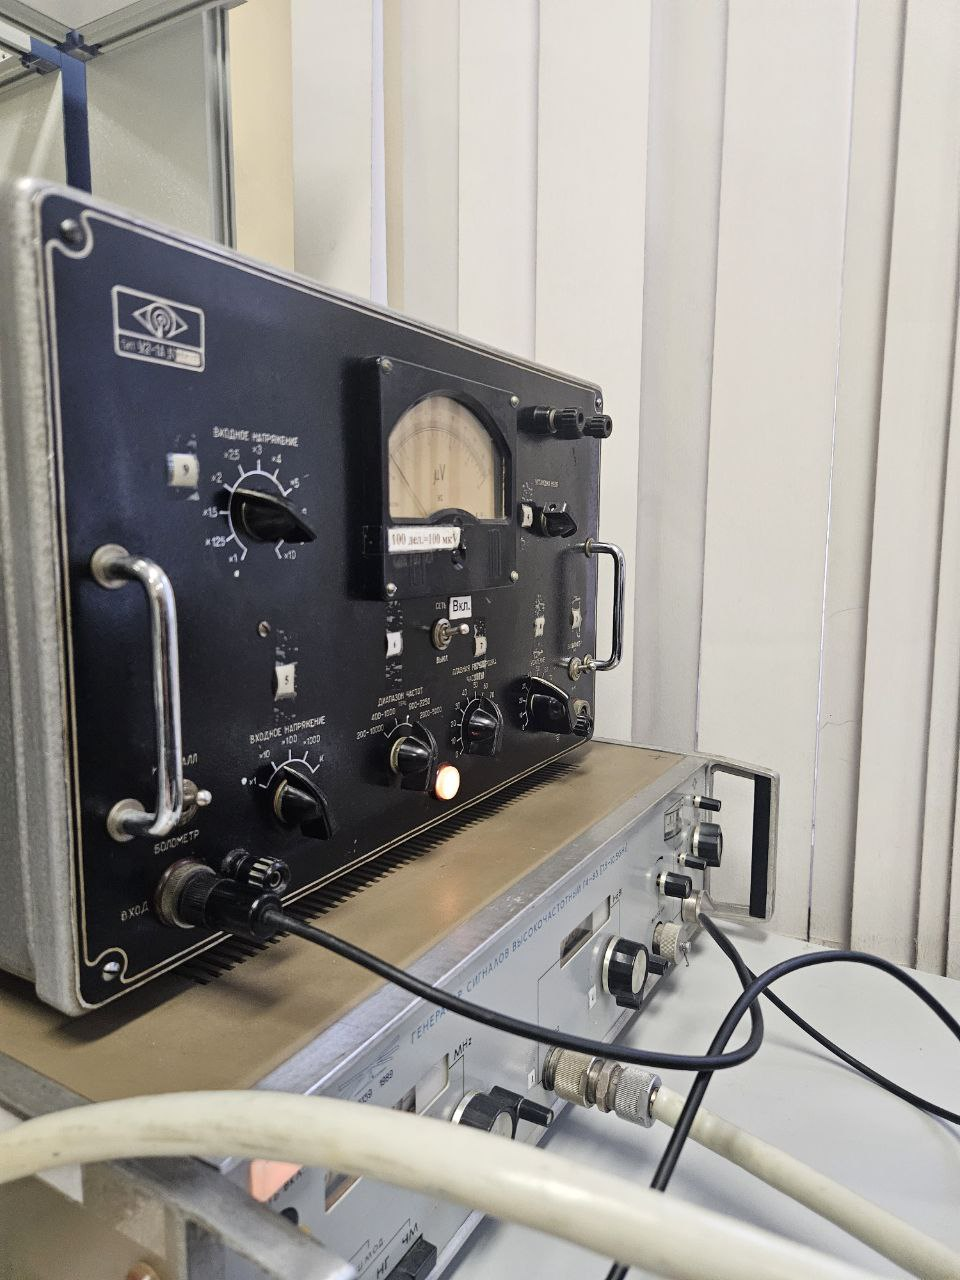
\includegraphics[scale=0.08]{photo_2024-12-24_17-45-34.jpg}
            \caption{Усилитель и генератор}
        \end{subfigure}
    \end{figure}
    
\end{frame}




\begin{frame}{Определение длины волны СВЧ-сигнала в волноводе при частоте выше критической}
    \begin{block}{}
        \centering
        Для нахождения длины волны в волноводе снимем зависимость напряжения от координаты зонда. Получим график зависимости U(z):
    \end{block}
    
    \begin{figure}
        \centering
        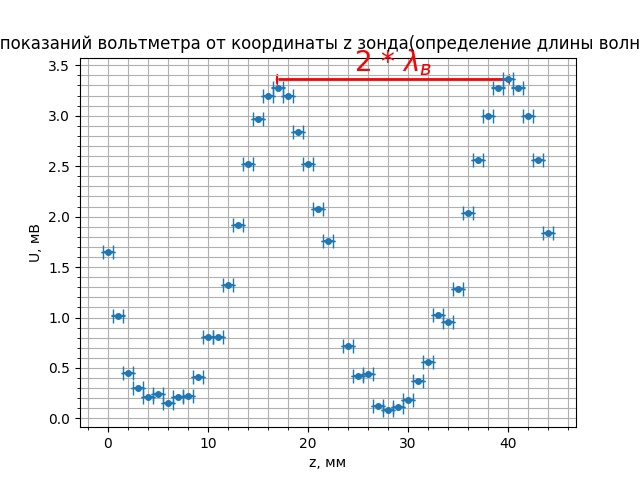
\includegraphics[scale=0.3]{graf11.jpg}
        \caption{Зависимость напряжения U от координаты z}
        \label{fig:enter-label}
    \end{figure}
\end{frame}
\begin{frame}{Определение длины волны СВЧ-сигнала в волноводе при частоте выше критической}

    \begin{block}{}
        \centering
        Половина длины волны в волноводе соответствует расстоянию между пиками графиков
    \end{block}

    \begin{block}{Длина волны в волноводе, измеренная экспериментально}
        \centering
        \begin{equation}
            \lambda = 46 \pm 0.5 \text{мм}
        \end{equation}
    \end{block} 

\end{frame}


\begin{frame}{Определение характера детектирования зонда}

    \begin{block}{}
        Как показано в теории, поле в волноводе $E \propto sin (k_z z)$. В узлах значения аргумента синуса малы, поэтому $E \propto z$
    \end{block}
    
    \begin{block}{}
        Устройство детекторной головки такого, что отклик вольтметра $U \propto E^n \propto z^n$, где n = 1 для больших сигналов и n = 2 для малых. Построим U(z) в логарифмическом масштабе, причем значения координат z будем брать около узла
    \end{block}
    
\end{frame}


\begin{frame}{Определение характера детектирования зонда}

    \begin{block}{}
        \centering
        По углу наклона кривой определим n
    \end{block}

    \begin{figure}[!h]
        \centering
        \begin{subfigure}{0.5\textwidth} % Задаем ширину подфигуры
            \centering
            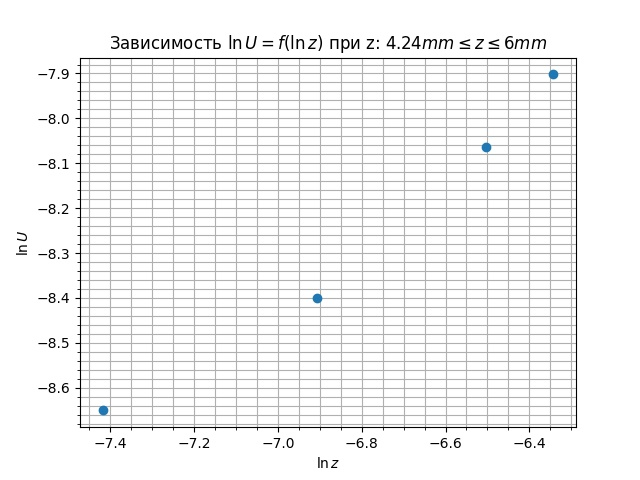
\includegraphics[scale=0.25]{1.jpg}
        \end{subfigure}
        \hfill
        \begin{subfigure}{0.48\textwidth} % Задаем ширину подфигуры
            \centering
            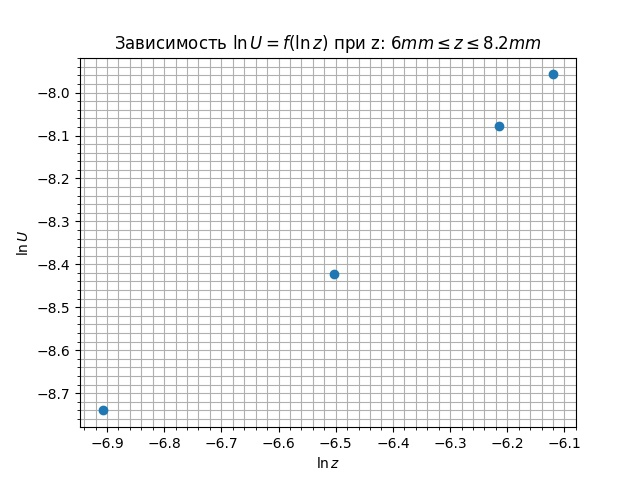
\includegraphics[scale=0.25]{2.jpg}
        \end{subfigure}
    \end{figure}

    \begin{block}{Характер детектирования}
        \centering
       Получим n приблизительно равное 1
    \end{block}

\end{frame}


\begin{frame}{Определение коэффициента отражения}

    \begin{block}{}
        Коэффициент отражения показывает, во сколько раз отличаются апмлитуды падающей и отраженной волн. Как было получено в файле с теорией, его удобно считать по следующей формуле:
    \end{block}

    \begin{block}{Коэффициент отражения}
        \begin{equation}
            \rho = \frac{E_{max} - E_{min}}{E_{max} + E_{min}}
        \end{equation}
    \end{block}

       
\end{frame}


\begin{frame}{Определение коэффициента отражения}

    \begin{block}{Теоретические ожидания}
        \begin{itemize}
            \item При наличии поглощающей нагрузки ожидаем, что волна полностью поглатиться, $E_{min} = E_{max} = E$, те E не зависит от координаты, $\rho = 0$
            \item При наличии металлической заглушки ожидаем полное отражение. В волноводе образуется стоячая волна, $E_{min} = 0$, $\rho = 1$
            \item При открытом конце волновода имеем бегущую волну.
        \end{itemize}
    \end{block}
    
\end{frame}

\begin{frame}{Определение коэффициента отражения}

    \begin{block}{Экспериментальные значения}
        \begin{itemize}
            \item $\rho_{opened} = 0.73 \pm 0.11$
            \item $\rho_{closed} = 0.51 \pm 0.09$
            \item $\rho_{load} = 0.11 \pm 0.03$
        \end{itemize}
    \end{block}


    \begin{block}{Обсуждение результатов}
        Можно видеть, что при наличии поглощающей нагрузки коэффициент отражения отличен от нуля, что, вероятно, говорит о неидельной 'стыковке' металлической заглушки и волновода - часть волны отражается от неровностей в месте соединения. При открытом конце, а при закрытом коэффициент 0.73.
    \end{block}

    
\end{frame}



\begin{frame}{Исследование затухания волн при частоте ниже критической}

    \begin{block}{}
        При частоте волны ниже критической ожидаем увидеть экспоненциальное затухание. Согласно теории, коэффициент ослабления связан с длиной волновода линейно - через коэффициент затухания: $\gamma = -\beta z$
    \end{block}

    \begin{block}{}
        Будем уменьшать длину волновода (последовательно уменьшая количество секций от 3-х до нуля), подбирая такой коэффициент ослабления с генератора, чтобы показания вольтметра на усилителе оставались постоянными
    \end{block}
    
\end{frame}


\begin{frame}{Исследование затухания волн при частоте ниже критической}

    \begin{block}{}
        Построим график $\gamma(z)$ и по его углу наклона найдем $\beta$
    \end{block}

    \begin{figure}
        \centering
        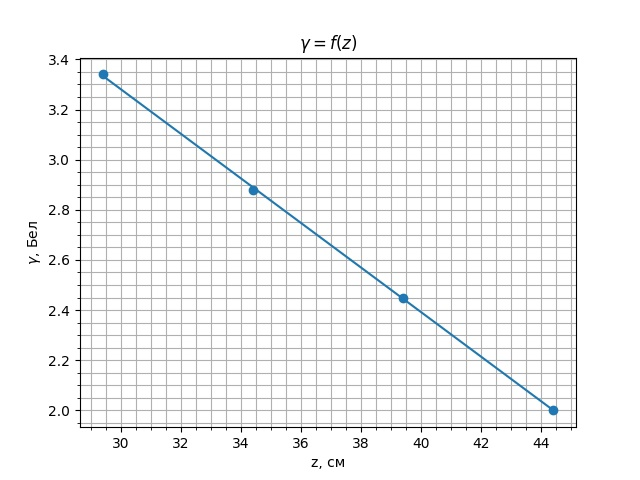
\includegraphics[scale=0.35]{graf33.jpg}
        \caption{Зависимость коэффициента ослабления от длины волновода}
        \label{fig:enter-label}
    \end{figure}

    \begin{block}{}
        \begin{equation}
            \beta = !!!! \pm!!!!
        \end{equation}
    \end{block}
    
\end{frame}


\begin{frame}{Результаты}

    \begin{block}{}
        \item 1. Получено значение длины волны в волноводе при частоте выше критической
        \item 2. Был подтвержден линейный характер детектирования зонда
        \item 3. Были определены коэффициенты отражения волны от металлической заглушки, воздушного пространства и при наличии поглащающей нагрузки (в последнем случае коэффициент отличен от нуля, что связано с неровности в месте стыковке волновода и нагрузки)
        \item 4. Был получен коэффициент затухания СВЧ-волн при частоте ниже критической
    \end{block}
    
\end{frame}


\end{document}